\documentclass{article}
\usepackage[english]{babel}
\usepackage[utf8]{inputenc}
\usepackage{fancyhdr}
\usepackage{geometry}
\usepackage{enumitem}
\usepackage{amsmath}
\usepackage{graphicx}
\usepackage{tcolorbox}
\usepackage{amssymb}
\usepackage[thinc]{esdiff}
\usepackage{float}

%%%%%%%%%%%%%%%%%%%%%%%%%%%%%%%%%%%%%%%%%%%%%%%%%%%%%%%%%%%%%%%%%%%%%%%%

\geometry{letterpaper, portrait, margin=1in}
\graphicspath{ {images/} }
\pagestyle{fancy}
\fancyhf{}
\lhead{Keerthik Muruganandam}
\rhead{Yadavalli Written Work X}

%%%%%%%%%%%%%%%%%%%%%%%%%%%%%%%%%%%%%%%%%%%%%%%%%%%%%%%%%%%%%%%%%%%%%%%%

\begin{document}

\begin{enumerate}[label=\textbf{(5.\arabic*)}]

%%%%%%%%%%%%%%%%%%%%%%%%%%%%%%%%%%%%%%%%%%%%%%%%%%%%%%%%%%%%%%%%%%%%%%%%

\item Use the substitution $u-\sec x$ to evaluate the integral $\displaystyle{\int\!\tan^7x\sec^3x\, dx}$.
%%%%%%%%%%%%%%%%%%%%%%%%%%%%%%%%%%%%%%%%%%%%%%%%%%%%%%%%%%%%%%%%%%%%%%%%

If we let $u=\sec x$, then $du=\sec x\tan x$.
\begin{align*}
    \int\!\tan^7x\sec^3x\, dx &= \int\!\tan^6x\sec^2x\cdot\tan x\sec x\, dx \\
    &=\int\!\tan^6x \,u^2\, du
\end{align*}
To remove the $\tan^6x$ in the integrand, we can utilize the identity $\tan^2x+1=\sec^2x$ to derive the equation $\tan^6x=\left(\sec^2x-1\right)^3$.
\begin{align*}
    \int\!\tan^6x \,u^2\, du &= \int\!\left(\sec^2x-1\right)^3u^2\, du \\ 
    &= \int\!\left(u^2-1\right)^3u^2\,du \\
    &= \int\!\left(u^8-3u^6+3u^4-u^2\right)
\end{align*}
Now the integrand is in a form which is easily integrated with the power rule
\begin{align*}
    \int\!\left(u^8-3u^6+3u^4-u^2\right) &= \frac{u^9}{9}-3\frac{u^7}{7}+3\frac{u^5}{5}-\frac{u^3}{3}+C \\
    &= \frac{\sec^9x}{9}-3\frac{\sec^7x}{7}+3\frac{\sec^5x}{5}-\frac{\sec^3x}{3}+C
\end{align*}
Thus we have found out final answer which is
\begin{center}
\fbox{$\displaystyle{\int\!\tan^7x\sec^3x\, dx}=\frac{\sec^9x}{9}-3\frac{\sec^7x}{7}+3\frac{\sec^5x}{5}-\frac{\sec^3x}{3}+C$} \\
\vspace{1 in}
Problem 2 on next page. $\rightarrow$
\end{center}

%%%%%%%%%%%%%%%%%%%%%%%%%%%%%%%%%%%%%%%%%%%%%%%%%%%%%%%%%%%%%%%%%%%%%%%%

\newpage 

%%%%%%%%%%%%%%%%%%%%%%%%%%%%%%%%%%%%%%%%%%%%%%%%%%%%%%%%%%%%%%%%%%%%%%%%

\item Evaluate the integral $\displaystyle{\int\!\frac{x^3}{\sqrt{x^2+1}}\,dx}$ using the following two methods.
\begin{enumerate}
    \item Use the substitution $u=x^2+1$.
    \item Use the substitution $x=\tan\theta$.
\end{enumerate}
%%%%%%%%%%%%%%%%%%%%%%%%%%%%%%%%%%%%%%%%%%%%%%%%%%%%%%%%%%%%%%%%%%%%%%%%

\begin{enumerate}
    \item Let $u=x^2+1$. Therefore, $du=2x$. Substitution into the integral looks like
    \begin{align*}
        \int\!\frac{x^3}{\sqrt{x^2+1}}\,dx &= \int\!\frac{2}{2}\frac{x^2}{\sqrt{x^2+1}}\,dx \\
        &= \int\!\frac{1}{2}\frac{x^2\cdot2x}{\sqrt{x^2+1}}\,dx \\
        &= \frac{1}{2}\int\!\frac{x^2}{\sqrt{u}}\,du
    \end{align*}
    Removal of the $x^2$ in the integrand can be accomplished using the equation $x^2=u-1$, which is a manipulation of $u=x^2+1$.
    \begin{align*}
        \frac{1}{2}\int\!\frac{x^2}{\sqrt{u}}\,du &= \frac{1}{2}\int\!\frac{u-1}{\sqrt{u}}\,du \\
        &= \frac{1}{2}\int\!u^{1/2}-u^{-1/2}\,du
    \end{align*}
    Now the integral is in a form which is easily integratable using the power rule.
    \begin{align*}
        \frac{1}{2}\int\!u^{1/2}-u^{-1/2}\,du &= \frac{u^{3/2}}{3}-\sqrt{u}+C \\
        &= \frac{{\left(x^2+1\right)}^{3/2}}{3}-\sqrt{x^2+1}+C
    \end{align*}
    Thus we have our answer that \fbox{$\displaystyle{\int}\!\dfrac{x^3}{\sqrt{x^2+1}}\,dx=\frac{{\left(x^2+1\right)}^{3/2}}{3}-\sqrt{x^2+1}+C$}
    
    \item If we set $x=\tan\theta$ and $dx=\sec^2\theta\,d\theta$, we can draw the following triangle using the the trigonometric identity $\tan\theta=\frac{opp}{adj}$. 
    \begin{figure}[H]
        \centering
        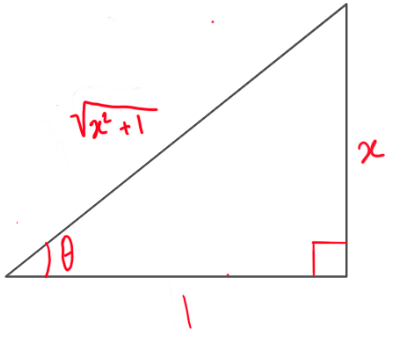
\includegraphics[width=5cm]{blurp}
    \end{figure}
    Now we can substitute in our values for $x$ and $dx$.
    \begin{align*}
        \int\!\frac{x^3}{\sqrt{x^2+1}}\,dx &= \int\!\frac{x^3\sec^2\theta}{\sqrt{\tan^2\theta+1}}\,d\theta \\
        &= \int\!\frac{\tan^3\theta\sec^2\theta}{\sqrt{\sec^2\theta}}\,d\theta \\
        &=\int\!\tan^3\theta\sec\theta\,d\theta
    \end{align*}
    Now we can use u substitution to solve this integral. Let $u=\sec\theta$ and $du=\sec\theta\tan\theta$. First we use the trig identity $\tan^2\theta=\sec^2\theta-1$ and then u substitution.
    \begin{align*}
        \int\!\tan^3\theta\sec\theta\,d\theta &= \int\!\left(\sec^2-1\right)\tan\theta\sec\theta\,d\theta \\
        &= \int\!u^2-1\,du
    \end{align*}
    Now we can evaluate the indefinite integral.
    \begin{align*}
        int\!u^2-1\,du &= \frac{u^3}{3}-u+C \\
        &= \frac{\sec^3\theta}{3}-\sec\theta+C
    \end{align*}
    We can find the value of $\sec\theta$ because $\sec\theta=\frac{hyp}{opp}$ which is equal to $\sqrt{x^2+1}$ from the triangle above. Therefore,
    \begin{align*}
        \frac{\sec^3\theta}{3}-\sec\theta+C &= \frac{{\left(\sqrt{x^2+1}\right)}^3}{3}-\sqrt{x^2+1}+C \\
    \end{align*}
    Since parts $(a)$ and $(b)$ are equal, we can safely conclude that
    \begin{center}
        \fbox{$\displaystyle{\int}\!\dfrac{x^3}{\sqrt{x^2+1}}\,dx=\frac{{\left(x^2+1\right)}^{3/2}}{3}-\sqrt{x^2+1}+C$}
    \end{center}
\end{enumerate}
\vspace{1 in}
\begin{center}
Problem 3 on next page. $\rightarrow$
\end{center}

%%%%%%%%%%%%%%%%%%%%%%%%%%%%%%%%%%%%%%%%%%%%%%%%%%%%%%%%%%%%%%%%%%%%%%%

\newpage

%%%%%%%%%%%%%%%%%%%%%%%%%%%%%%%%%%%%%%%%%%%%%%%%%%%%%%%%%%%%%%%%%%%%%%%

\item Evaluate the integral $\displaystyle{\int\!\frac{x^2}{x^2+9}\,dx}$ and draw a triangle according to your trig substitution.
%%%%%%%%%%%%%%%%%%%%%%%%%%%%%%%%%%%%%%%%%%%%%%%%%%%%%%%%%%%%%%%%%%%%%%%%

To start, let us determine what side length we are looking for. The integral has a denominator of $x^2+9$ so we look for a triangle which has that to some power on a side. The triangle that fulfills that requirement is
\begin{figure}[H]
    \centering
    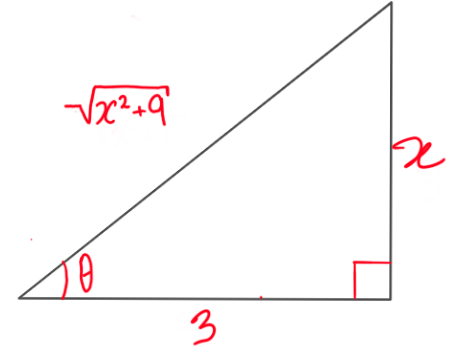
\includegraphics[width=5cm]{sines}
\end{figure}
Thus we can tell that our substitution is $x=3\tan\theta$ and $du=3\sec^2\theta\,d\theta$.
\begin{align*}
\int\!\frac{x^2}{x^2+9}\,dx &= \int\!\frac{9\tan^2\theta3\sec^2\theta}{9\tan^2\theta+9}\,d\theta \\
&= \int\!\frac{3\tan^2\theta\sec^2\theta}{\tan^2\theta+1}\,d\theta \\
&= \int\!\frac{3\tan^2\theta\sec^2\theta}{\sec^2\theta}\,d\theta \\
&= 3\int\!\tan^2\theta\,d\theta
\end{align*}
Now we can evaluate the integral because of the identity $\tan^2\theta=\sec^2\theta-1$.
\begin{align*}
    3\int\!\tan^2\theta\,d\theta&=3\int\!\sec^2\theta-1\,d\theta \\
    &=3\left(\int\!\sec^2\theta\,d\theta-\int\!1\,d\theta\right) \\
    &=3\left(\tan\theta-\theta+C\right)
\end{align*}
Now we have to re-substitute in the values for $\theta$. Using our value for $x$ we find that $\theta=\arctan\left(\frac{x}{3}\right)$.
\begin{align*}
    3\left(\tan\theta-\theta+C\right) &= 3\left(\frac{x}{3}-\arctan\left(\frac{x}{3}\right)+C \right) \\
    &= x-3\arctan\left(\frac{x}{3}\right)
\end{align*}
That is the final answer to our problem
\begin{center}
    \fbox{$\displaystyle{\int\!\frac{x^2}{x^2+9}\,dx=x-3\arctan\left(\frac{x}{3}\right)}$} \\
    \vspace{1 in}
    Problem 4 on next page. $\rightarrow$
\end{center}

%%%%%%%%%%%%%%%%%%%%%%%%%%%%%%%%%%%%%%%%%%%%%%%%%%%%%%%%%%%%%%%%%%%%%%%

\newpage

%%%%%%%%%%%%%%%%%%%%%%%%%%%%%%%%%%%%%%%%%%%%%%%%%%%%%%%%%%%%%%%%%%%%%%%

\item \textbf{Professional Problem:} Define $G(n)=\int_0^\infty\!x^ne^{-x}\,dx$.
\begin{enumerate}
    \item Show $G(n)=nG(n-1)$ for $n\geq1$.
    \item Let $n$ be a positive integer. Explain why $G(n)=n!$.
\end{enumerate}
%%%%%%%%%%%%%%%%%%%%%%%%%%%%%%%%%%%%%%%%%%%%%%%%%%%%%%%%%%%%%%%%%%%%%%%%

If we use IBP on  the indefinite integral form of $G(n)$ with a $u=x^n$ and a $dv=e^{-x}\,dx$, we create the equation
\begin{align}
        \int\!x^ne^{-x}\,dx &= -x^ne^{-x}+n\int\!x^{n-1}e^{-x}\,dx+C\mathrm{.}
    \end{align} %First Integral
Notice that $\int\!x^{n-1}e^{-x}\,dx=G(n-1)$. We can see from this that the integral will keep repeating until we reach $G(1)$. Recalling the groupwork Alternative Factorials, we know that $G(1)=1$ Thus, the integral is actually
\begin{align}
    \int\!x^ne^{-x}\,dx &= \left(-x^ne^{-x}-nx^{n-1}e^{-x}\ldots-e^{-x}\right)+n!+C\mathrm{.}
\end{align} %n! form created
Now we have the complete antiderivative we can evaluate $G(n)$ by finding the limit as $x$ approaches $\infty$ of the integral from $0$ to $t$. This yields the equations
\begin{align}
    \left[\left(-x^ne^{-x}-nx^{n-1}e^{-x}\ldots-e^{-x}\right)+n!\right]_0^t &= \left(-t^ne^{-t}-nt^{n-1}e^{-t}\ldots-e^{-t}\right)+n!
\end{align}
Now to take the limit of this expression we can again utilize the groupwork, where we showed that $\lim_{x\to\infty} \dfrac{x^n}{e^{x}}=0$. By this logic, everything within parentheses should equal $0$. Applying the limit gives us
\begin{align*}
    \lim_{t\to\infty} {\left(-t^ne^{-t}-nt^{n-1}e^{-t}\ldots-e^{-t}\right)+n!} &= \lim_{x\to\infty} {\left(-t^ne^{-t}-nt^{n-1}e^{-t}\ldots-e^{-t}\right)}+\lim_{x\to\infty} {n!} \\ 
    &= 0+n!\lim_{x\to\infty} {1} \\
    &= n!\mathrm{.}
\end{align*}
Thus we can see that $G(n)=n!$ for a positive $n$. We can also conclude that $G(n)=nG(n-1)$ for $n\geq1$ because 
\begin{align*}
    G(n) &= nG(n-1) \\
    &=n\cdot(n-1)! \\
    &=n! \\
    &= G(n)\mathrm{.}
\end{align*}
We have concluded that $G(n)=nG(n-1)$ for $n\geq1$ and $G(n)=n!$ when $n$ is a positive integer.

%%%%%%%%%%%%%%%%%%%%%%%%%%%%%%%%%%%%%%%%%%%%%%%%%%%%%%%%%%%%%%%%%%%%%%%

\end{enumerate}

\end{document}
